%%% PostgreSQL Conference Europe 2013, Dublin, Oct 29, 2013
%%%
%%% What extensions are available? Where do you get them from? How to write
%%% Extensions, including portability, multi-version compatibility and
%%% controls. Includes discussion of new 9.3 feature background workers.

\documentclass{beamer}

\usepackage[utf8]{inputenc}

\usepackage{minted}

\usepackage{beamerthemesplit}
\usetheme{Boadilla}
%\setbeamertemplate{itemize items}{\checkmark}
\setbeamertemplate{itemize items}[circle]
\beamertemplatetransparentcovered

\usepackage{multicol}

\title{Writing \& using Postgres Extensions}
\subtitle{PostgreSQL Conference Europe 2013}
\author{Dimitri Fontaine \texttt{dimitri@2ndQuadrant.fr}}
\date{October, 29 2013}
\logo{
\includegraphics[height=0.4cm]{2ndQuadrant-cross.png}}

\begin{document}

\frame{\titlepage}

\begin{frame}[fragile]
  \frametitle{Dimitri Fontaine}

  \begin{center}
    \textbf{2ndQuadrant France}
    \linebreak
    PostgreSQL Major Contributor
  \end{center}
  \vfill

\begin{columns}[c]
\column{.75\textwidth} 

  \begin{itemize}
   \item \texttt{pgloader}, \texttt{prefix}, \texttt{skytools}, …
   \item \texttt{apt.postgresql.org}
   \item \texttt{\textbf{CREATE EXTENSION}}
   \item \texttt{\textbf{CREATE EVENT TRIGGER}}
   \item MySQL migration tool, new \texttt{pgloader} version
  \end{itemize}  

\column{.25\textwidth}
\begin{center}
  
\includegraphics[height=7em]{2ndQuadrant-cross.png}
\end{center}
\end{columns}
\end{frame}

\section{PostgreSQL Extensibility}

\begin{frame}[fragile]
  \frametitle{PostgreSQL Extensibility}

  \center{PostgreSQL is \textit{highly} \textbf{extensible}}
  \vfill

\begin{center}
  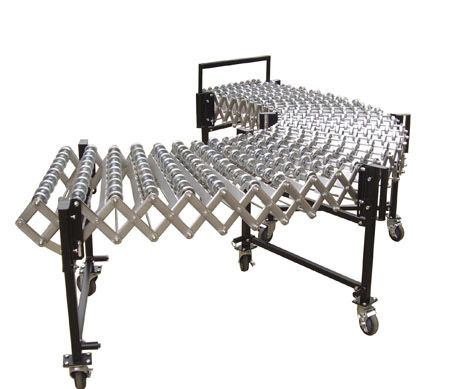
\includegraphics[height=15em]{extensible.jpg}
\end{center}
\end{frame}

\begin{frame}[fragile]
  \frametitle{PostgreSQL Extensibility}

\begin{minted}{postgresql}
select col1, col2 from table where col1 = 'something';

  SELECT col
    FROM table
   WHERE stamped > date 'today' - interval '1 day';

\end{minted}
\end{frame}

\begin{frame}[fragile]
  \frametitle{PostgreSQL Extensibility}

\begin{minted}{postgresql}
select actor from products where actor % 'tomy';
\end{minted}
\end{frame}

\begin{frame}[fragile]
  \frametitle{PostgreSQL Extensibility}

\begin{minted}{postgresql}
    select name,
           pos <@> point(-0.12,51.516) as miles
      from pubnames
  order by pos <-> point(-0.12,51.516) desc
     limit 5;
\end{minted}
\end{frame}

\begin{frame}[fragile]
  \frametitle{PostgreSQL Extensibility}

\begin{minted}{postgresql}
   select id, name, pos,
          pos <@> point(-0.12,51.516) as miles
     from pubnames
 order by pos <-> point(-0.12,51.516)
    limit 10;
\end{minted}
\end{frame}

\begin{frame}[fragile]
  \frametitle{PostgreSQL Extensibility}

\begin{minted}{postgresql}
with geoloc as (
    select location
      from geolite.location l
           join geolite.blocks using(locid)
     where iprange >>= '212.58.251.195'
)
    select name,
           pos <@> (select location from geoloc) as miles
      from pubnames
  order by pos <-> (select location from geoloc)
     limit 10;
\end{minted}
\end{frame}

\begin{frame}[fragile]
  \frametitle{PostgreSQL is Extensible}

  \center{PostgreSQL plugins are data types and index support}
  \vfill

\begin{columns}[c]
\column{.55\textwidth} 

  \begin{itemize}
  \item Data Type
  \item Input/Output functions
  \item Casts
  \item Operator Classes
  \end{itemize}

\column{.45\textwidth}
\begin{center}
  
\includegraphics[height=12em]{plus-equal-sign-1024x1024.jpg}
\end{center}
\end{columns}
\end{frame}

\begin{frame}[fragile]
  \frametitle{PostgreSQL is Extensible}

  \center{PostgreSQL support several kind of indexes}
  \vfill

\begin{columns}[c]
\column{.55\textwidth} 

  \begin{itemize}
  \item BTree, binary tree
  \item GiST, Generalized Search Tree
  \item SP-GiST, Space Partitioned GiST
  \item GIN, Generalized Inverted Index
  \end{itemize}

\column{.45\textwidth}
\begin{center}
  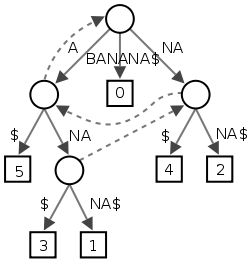
\includegraphics[height=12em]{suffix-tree-banana.png}
\end{center}
\end{columns}
\end{frame}


\begin{frame}[fragile]
  \frametitle{Binary Tree}

  \center{Btree, the default index type}
  \vfill

\begin{columns}[c]
\column{.55\textwidth} 

  \begin{itemize}
  \item Built for speed
  \item \textit{unique} concurrency tricks
  \item Balanced
  \item support function: \texttt{cmp}
  \item operators: \texttt{<= < = > >=}
  \end{itemize}

\column{.45\textwidth}
\begin{center}
  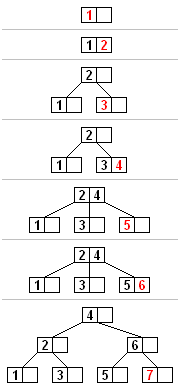
\includegraphics[height=14em]{B_tree_insertion_example.png}
\end{center}
\end{columns}
\end{frame}


\begin{frame}[fragile]
  \frametitle{Generalized Index Search Tree}

  \center{GiST or the Indexing API}
  \vfill

\begin{columns}[c]
\column{.55\textwidth} 

  \begin{itemize}
  \item Built for comfort
  \item Balanced
  \item API: \texttt{consistent}, \texttt{same}, \texttt{union}
  \item API: \texttt{penalty}, \texttt{picksplit}
  \item API: \texttt{compress}, \texttt{decompress}
  \item operators: \texttt{@> <@ \&\& @@ = \&< \&> <<| ...}
  \end{itemize}

\column{.45\textwidth}
\begin{center}
  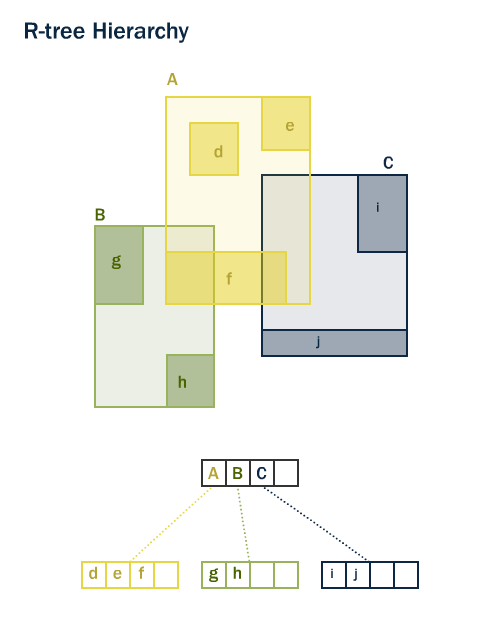
\includegraphics[height=14em]{rtree.png}
\end{center}
\end{columns}
\end{frame}


\begin{frame}[fragile]
  \frametitle{Generalized Inverted iNdex}

  \center{Indexing several pointers per value, inversed cardinality}
  \vfill

\begin{columns}[c]
\column{.55\textwidth} 

  \begin{itemize}
  \item Built for Text Search and Arrays
  \item Balanced
  \item API: \texttt{compare}, \texttt{consistent}
  \item API: \texttt{extractValue}, \texttt{extractQuery}
  \item operators: \texttt{@> <@ \&\& =}
  \end{itemize}

\column{.45\textwidth}
\begin{center}
  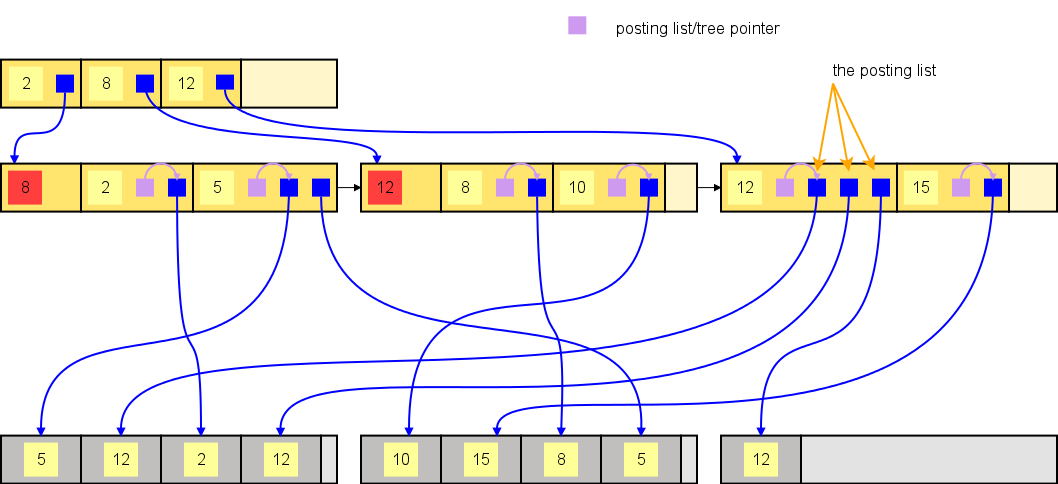
\includegraphics[height=5em]{gin.png}
\end{center}
\end{columns}
\end{frame}

\section{Extensions}

\begin{frame}[fragile]
  \frametitle{Extensions and data types}

\begin{center}
  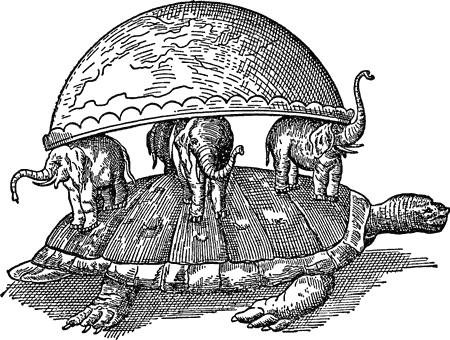
\includegraphics[height=18em]{extensions.png}
\end{center}
\end{frame}

\begin{frame}[fragile]
  \frametitle{Some extensions example}

  \center{46 Contribs, Community extensions, Private ones...}
  \vfill

\begin{columns}[c]

\column{.18\textwidth}
  \begin{itemize}
   \item cube
   \item \alert{ltree}
   \item citext
   \item \alert{hstore}
   \item \alert{intagg}
  \end{itemize}

\column{.25\textwidth}
  \begin{itemize}
   \item \alert{earthdistance}
   \item pgq
   \item \alert{pg\_trgm}
   \item wildspeed
   \item \alert{plproxy}
  \end{itemize}

\column{.21\textwidth} 
  \begin{itemize}
   \item PostGIS
   \item \alert{ip4r}
   \item \alert{hll}
   \item \alert{prefix}
   \item pgfincore
  \end{itemize}

\column{.4\textwidth}
  \begin{itemize}
   \item pgcrypto
   \item pg\_stattuple
   \item pg\_buffercache
   \item pg\_stat\_statements
   \item \alert{pgfincore}
  \end{itemize}

\end{columns}
\end{frame}

\section{HyperLogLog}

\begin{frame}[fragile]
  \frametitle{HyperLogLog}

  \center{State of The Art Cardinality Estimation Algorithm}
  \vfill

\begin{center}
  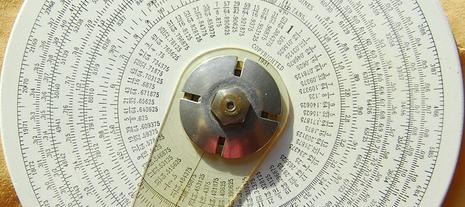
\includegraphics[height=12em]{cardinality1.jpg}
\end{center}
\end{frame}

\begin{frame}[fragile]
  \frametitle{Creating the unique visitors tracking table}

\begin{minted}{postgresql}
CREATE EXTENSION hll;

-- Create the destination table
CREATE TABLE daily_uniques (
    DATE            DATE UNIQUE,
    users           hll
);

-- Our first aggregate update
UPDATE daily_uniques
   SET users = hll_add(users,
                 hll_hash_text('123.123.123.123'))
 WHERE date = current_date;
\end{minted}  
\end{frame}

\begin{frame}[fragile]
  \frametitle{Production ready updates}

\begin{minted}{postgresql}
--
-- First upload a new batch, e.g. using
--    CREATE TEMP TABLE new_batch as VALUES(), (), ...;
--
WITH hll(agg) AS (
 SELECT hll_add_agg(hll_hash_text(value))
   FROM new_batch
)
 UPDATE daily_uniques
    SET users = CASE WHEN hll.agg IS NULL THEN users
                     ELSE hll_union(users, hll.agg)
                 END
   FROM hll
  WHERE date = current_date;
\end{minted}  
\end{frame}

\begin{frame}[fragile]
  \frametitle{Daily Reporting}

\begin{minted}{postgresql}
with stats as (
  select date, #users as daily,
         #hll_union_agg(users) over() as total
    from daily_uniques
)
  select date,
         round(daily) as daily,
         round((daily/total*100)::numeric, 2) as percent
    from stats
order by date;
    date    | daily  | percent 
------------+--------+---------
 2013-02-22 | 401677 |   25.19
 2013-02-23 | 660187 |   41.41
 2013-02-24 | 869980 |   54.56
 2013-02-25 | 154996 |    9.72
(4 rows)
\end{minted}  
\end{frame}

\begin{frame}[fragile]
  \frametitle{Monthly Reporting}

\begin{minted}{postgresql}
   select to_char(date, 'YYYY/MM') as month,
          round(#hll_union_agg(users)) as monthly
     from daily_uniques group by 1;
     
  month  | monthly 
---------+---------
 2013/02 | 1960380
(1 row)
\end{minted}  
\end{frame}

\section{Earth Distance}

\begin{frame}[fragile]
  \frametitle{Earth Distance}

\begin{center}
  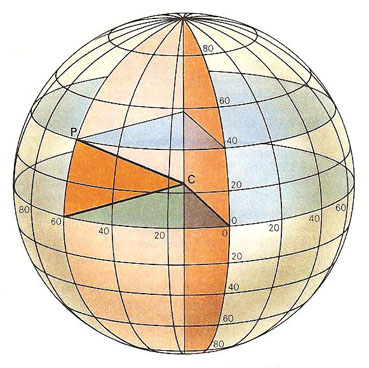
\includegraphics[height=15em]{latitude_and_longitude.jpg}
\end{center}
\end{frame}

\begin{frame}[fragile]
  \frametitle{How Far is The Nearest Pub}

  \center{The \texttt{point} datatype is in-core}
  \vfill

\begin{minted}{postgresql}
#  CREATE TABLE pubnames (id bigint, pos POINT, name text);

#  select name, pos
     from pubnames
 order by pos <-> point(-0.12,51.516)
    limit 3;

          name          |           pos           
------------------------+-------------------------
 All Bar One            | (-0.1192746,51.5163499)
 The Shakespeare's Head | (-0.1194731,51.5167871)
 The Newton Arms        | (-0.1209811,51.5163032)
(3 rows)

Time: 18.679 ms
\end{minted}  
\end{frame}

\begin{frame}[fragile]
  \frametitle{How Far is The Nearest Pub}

  \center{KNN indexing is in core too!}
  \vfill

\begin{minted}{postgresql}
#  CREATE INDEX on pubnames USING GIST(pos);

#  select name, pos
     from pubnames
 order by pos <-> point(-0.12,51.516)
    limit 3;

          name          |           pos           
------------------------+-------------------------
 All Bar One            | (-0.1192746,51.5163499)
 The Shakespeare's Head | (-0.1194731,51.5167871)
 The Newton Arms        | (-0.1209811,51.5163032)
(3 rows)

Time: 0.849 ms
\end{minted}  
\end{frame}

\begin{frame}[fragile]
  \frametitle{How Far is The Nearest Pub, in Miles please.}

\begin{minted}{postgresql}
#  create extension cube;
#  create extension earthdistance;

#  select name,
 round((pos <@> point(-0.12,51.516))::numeric, 3) as miles
     from pubnames
 order by pos <-> point(-0.12,51.516)
    limit 10;
          name          | miles 
------------------------+-------
 All Bar One            | 0.039
 The Shakespeare's Head | 0.059
 The Newton Arms        | 0.047
(3 rows)

Time: 1.335 ms
\end{minted}  
\end{frame}

\begin{frame}[fragile]
  \frametitle{Some pubs far away from a random London based location.}

\begin{minted}{postgresql}
#   select c.name as city, p.name,
           round((pos <@> point(-0.12,51.516))::numeric, 3) as miles
      from pubnames p,
           lateral (select name
                      from cities c
                  order by c.pos <-> p.pos
                     limit 1) c
  order by pos <-> point(-0.12,51.516) desc
     limit 5;
  city  |      name       |  miles  
--------+-----------------+---------
 Galway | Tig Bhric       | 440.194
 Galway | TP's            | 439.779
 Galway | Begley's        | 439.752
 Galway | Ventry Inn      | 438.962
 Cork   | Fisherman's Bar | 439.153
(5 rows)

Time: 636.445 ms
\end{minted}  
\end{frame}

\section{HStore}

\begin{frame}[fragile]
  \frametitle{HStore}

\begin{center}
  
\includegraphics[height=9em]{hstore.png}
\end{center}
\end{frame}

\section{Trigrams}

\begin{frame}[fragile]
  \frametitle{Trigrams}

\begin{center}
  
\includegraphics[height=12em]{trigramme.png}
\end{center}
\end{frame}

\section{IP Ranges with ip4r}

\begin{frame}[fragile]
  \frametitle{IP Ranges, \texttt{ip4r}}

\begin{center}
  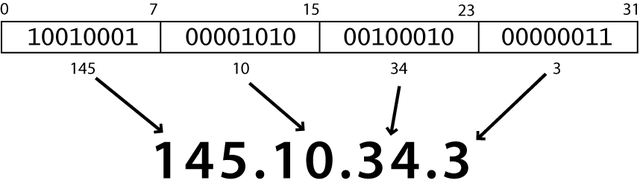
\includegraphics[height=6em]{ip-address.png}
\end{center}
\end{frame}

\section{plproxy}

\begin{frame}[fragile]
  \frametitle{\texttt{PL/Proxy}}

\begin{center}
  
\includegraphics[height=18em]{distribution.jpg}
\end{center}
\end{frame}


\section{base64}

\begin{frame}[fragile]
  \frametitle{Let's make a new one!}

\begin{center}
  
\includegraphics[height=18em]{extension-update.png}
\end{center}
\end{frame}

\begin{frame}[fragile]
  \frametitle{Packaging an extension}

\begin{center}
  
\includegraphics[height=18em]{software-upgrade.png}
\end{center}
\end{frame}

\begin{frame}[fragile]
  \frametitle{Packaging an extension}

  \center{We need a Makefile}
  \vfill

\begin{minted}{make}
EXTENSION   = base64
MODULES     = base64

LDFLAGS=-lrt

PG_CONFIG ?= pg_config
PGXS = $(shell $(PG_CONFIG) --pgxs)
include $(PGXS)
\end{minted}
\end{frame}

\frame{
  \frametitle{Questions?}

\begin{center}
  Now is the time to ask!
  \vfill

  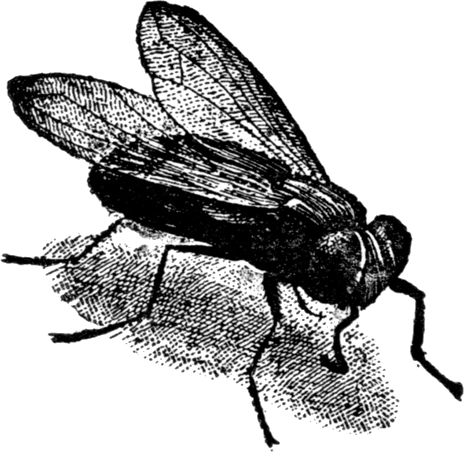
\includegraphics[height=9em]{fly.png}
\end{center}
}

\end{document}
